\section{Parametric Equations}\label{sec:param_eqs}

We are familiar with sketching  shapes, such as parabolas, by following this basic procedure:

\[
\begin{gathered}\text{Choose}\\x\end{gathered}
\longrightarrow
\begin{gathered}
\text{Use a function}\\f\text{ to find }y\\\bigl(y=f(x)\bigr)
\end{gathered}
\longrightarrow
\begin{gathered}\text{Plot point}\\(x,y)\end{gathered}
\]

In the rectangular coordinate system, the \textbf{rectangular equation} $y=f(x)$ works well for some shapes like a parabola with a vertical axis of symmetry, but in Precalculus and the review of conic sections in \autoref{sec:conic_sections}, we encountered several shapes that could not be sketched in this manner. (To plot an ellipse using the above procedure, we need to plot the ``top'' and ``bottom'' separately.)\index{curve!rectangular equation}

In this section we introduce a new sketching procedure:

\ifbool{latexml}{
\[
\begin{gathered}\text{Choose}\\t\end{gathered}\quad
\begin{gathered}
\rotatebox{-20}{\scalebox{2}{$\nearrow$}}\\
\rotatebox{20}{\scalebox{2}{$\searrow$}}
\end{gathered}\quad
{\addtolength{\jot}{-.5ex}
\begin{gathered}
\text{Use a function}\\f\text{ to find }x\\\bigl(x=f(t)\bigr)\\~\\
\text{Use a function}\\g\text{ to find }y\\\bigl(y=g(t)\bigr)
\end{gathered}
}\quad
\begin{gathered}
\rotatebox{20}{\scalebox{2}{$\searrow$}}\\
\rotatebox{-20}{\scalebox{2}{$\nearrow$}}
\end{gathered}\quad
\begin{gathered}\text{Plot point}\\(x,y)\end{gathered}
\]
}{
\begin{center}
\pdftooltip{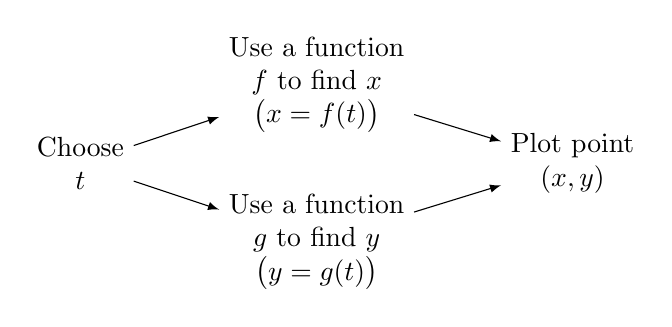
\begin{tikzpicture}[>=latex]
\draw (0,0) node (A) [align=center] {Choose \\$t$} 
      (3,1) node[align=center] (B1) {Use a function\\ $f$ to find $x$\\$\bigl(x=f(t)\bigr)$}
			(3,-1) node[align=center] (B2) {Use a function\\ $g$ to find $y$\\$\bigl(y=g(t)\bigr)$}
			(6.25,0) node [align=center] (C) {Plot point \\ $(x,y)$};
\draw [->](A) --(B1);
\draw [->](A) --(B2);
\draw [->](B1) -- (C);
\draw [->](B2) -- (C);
\end{tikzpicture}}{ALT-TEXT-TO-BE-DETERMINED}
\end{center}
}

Here, $x$ and $y$ are found separately but then plotted together. This leads us to a definition.

\begin{definition}[Parametric Equations and Curves]\label{def:param_eq}%%
Let $f$ and $g$ be continuous functions on an interval $I$. The \textbf{graph} of the \textbf{parametric equations} $x=f(t)$ and $y=g(t)$ is the set of all points $\bigl(x,y\bigr) = \bigl(f(t),g(t)\bigr)$ in the Cartesian plane, as the \textbf{parameter} $t$ varies over $I$. A \textbf{curve} is a graph along with the parametric equations that define it.
\index{curve!parametrically defined}\index{parametric equations!definition}
\end{definition}

\youtubeVideo{9kKZHQtYP7g}{Parametric Equations --- Some basic questions}

This is a formal definition of the word \emph{curve}. When a curve lies in a plane (such as the Cartesian plane), it is often referred to as a \textbf{plane curve}. Examples will help us understand the concepts introduced in the definition.

\mtable[-.5in]{A table of values of the parametric equations in \autoref{ex_pareq1} along with a sketch of their graph.}{fig:pareq1}{%
\tagpdfsetup{table/header-rows={1}}
\begin{tabular}{r @{\hspace{2em}} rr}
$t$ & $x$ & $y$ \\ \midrule
$-2$ & \phantom{$-$}4 & $-1$ \\
$-1$ & 1 & 0 \\
0 & 0 & 1 \\
1 & 1 & 2 \\
2 & 4 & 3
\end{tabular}\\(a)\\
\pdftooltip{\begin{tikzpicture}
\begin{axis}[width=1.16\marginparwidth,tick label style={font=\scriptsize},
axis y line=middle,axis x line=middle,name=myplot,
ymin=-2.2,ymax=4.2,xmin=-.9,xmax=5.2]
\addplot [thick,draw={\colorone}, smooth,domain=-2:2,] ({x^2},{x+1});
\draw [->,>=latex] (axis cs:3.9204,2.98) -- (axis cs:3.96,2.99);
\draw [->,>=latex] (axis cs:2.25,-.5) -- (axis cs:2.22,-.49);
\filldraw (axis cs:4,-1) circle (1.5pt) node [below] {\scriptsize $t=-2$};
\filldraw (axis cs:1,0) circle (1.5pt) node [shift={(0pt,-10pt)}]
 {\scriptsize $t=-1$};
\filldraw (axis cs:0,1) circle (1.5pt) node [left] {\scriptsize $t=0$};
\filldraw (axis cs:1,2) circle (1.5pt) node [above] {\scriptsize $t=1$};
\filldraw (axis cs:4,3) circle (1.5pt) node [above ] {\scriptsize $t=2$};
\end{axis}
\node [right] at (myplot.right of origin) {\scriptsize $x$};
\node [above] at (myplot.above origin) {\scriptsize $y$};
\end{tikzpicture}}{ALT-TEXT-TO-BE-DETERMINED}
\\(b)}

\begin{example}[Plotting parametric functions]\label{ex_pareq1}%%
Plot the graph of the parametric equations $x=t^2$, $y=t+1$ for $t$ in $[-2,2]$.
\solution
We plot the graphs of parametric equations in much the same manner as we plotted graphs of functions like $y=f(x)$: we make a table of values, plot points, then connect these points with a ``reasonable'' looking curve. \autoref{fig:pareq1}(a) shows such a table of values; note how we have 3 columns.

The points $(x,y)$ from the table are plotted in \autoref{fig:pareq1}(b). The points have been connected with a smooth curve. Each point has been labeled with its corresponding $t$-value. These values, along with the two arrows along the curve, are used to indicate the \textbf{orientation} of the graph. This information describes the \textbf{path} of a particle traveling along the curve.
\end{example}

We often use the letter $t$ as the parameter as we often regard $t$ as representing \emph{time}. Certainly there are many contexts in which the parameter is not time, but it can be helpful to think in terms of time as one makes sense of parametric plots and their orientation (for instance, ``At time $t=0$ the position is $(1,2)$ and at time $t=3$ the position is $(5,1)$.'').

\begin{example}[Plotting parametric functions]\label{ex_pareq2}%
%
\mtable{A table of values of the parametric equations in \autoref{ex_pareq2} along with a sketch of their graph.}{fig:pareq2}{%
\tagpdfsetup{table/header-rows={1}}
\begin{tabular}{c @{\hspace{2em}} cc}
$t$ & $x$ & $y$ \\ \hline
0 & 1 & 2 \\
$\pi/4$ & $1/2$ & $1+\sqrt{2}/2$ \\
$\pi/2$ & 0 & 1\\
$3\pi/4$ & $1/2$ & $1-\sqrt{2}/2$ \\
$\pi$ & 1 & 0
\end{tabular}
\\(a)\\
\pdftooltip{\begin{tikzpicture}
\begin{axis}[width=1.16\marginparwidth,tick label style={font=\scriptsize},
axis y line=middle,axis x line=middle,name=myplot,
ymin=-.1,ymax=2.1,xmin=-.1,xmax=1.6]
\addplot [thick,draw={\colorone}, smooth,domain=0:180,] ({(cos(x))^2},{cos(x)+1});
\draw [->,>=latex] (axis cs:0.998271, 0.00086485) -- (axis cs:0.999534, 0.000233112);
\draw [->,>=latex] (axis cs:0.770151, 1.87758) -- (axis cs:0.75311, 1.86782);
\filldraw (axis cs:1,2) circle (1.5pt) node [right] {\scriptsize $t=0$};
\filldraw (axis cs:.5,1.71) circle (1.5pt) node [below right]
 {\scriptsize $t=\pi/4$};
\filldraw (axis cs:0,1) circle (1.5pt) node [right] {\scriptsize $t=\pi/2$};
\filldraw (axis cs:.5,.292) circle (1.5pt) node [above right]
 {\scriptsize $t=3\pi/4$};
\filldraw (axis cs:1,0) circle (1.5pt) node [above right] {\scriptsize $t=\pi$};
\end{axis}
\node [right] at (myplot.right of origin) {\scriptsize $x$};
\node [above] at (myplot.above origin) {\scriptsize $y$};
\end{tikzpicture}}{ALT-TEXT-TO-BE-DETERMINED}
\\(b)}
%
Sketch the graph of the parametric equations $x=\cos^2t$, $y=\cos t+1$ for $t$ in $[0,\pi]$.
\solution
We again start by making a table of values in \autoref{fig:pareq2}(a), then plot the points $(x,y)$ on the Cartesian plane in \autoref{fig:pareq2}(b).

The curves in Examples \ref{ex_pareq1} and \ref{ex_pareq2} are portions of the same parabola $(y-1)^2+x=1$. While the \emph{parabola} is the same, the \emph{curves} are different. In \autoref{ex_pareq1}, if we let $t$ vary over all real numbers, we'd obtain the entire parabola. In this example, letting $t$ vary over all real numbers would still produce the same graph; this portion of the parabola would be traced, and re-traced, infinitely often. The orientation shown in \autoref{fig:pareq2} shows the orientation on $[0,\pi]$, but this orientation is reversed on $[\pi,2\pi]$.
\end{example}

\subsection{Converting between rectangular and parametric equations}

It is sometimes useful to transform rectangular form equations (i.e., $y=f(x)$) into parametric form equations, and vice-versa. Converting from rectangular to parametric can be very simple: given $y=f(x)$, the parametric equations $x=t$, $y=f(t)$ produce the same graph. As an example, given $y=x^2-x-6$, the parametric equations $x=t, y=t^2-t-6$ produce the same parabola. However, other parameterizations can be used. The following example demonstrates one possible alternative.

\mtable{The equation $f(x)=x^2-x-6$ with different parameterizations.}{fig_parab_param}{\pdftooltip{\begin{tikzpicture}
 \begin{axis}[width=1.16\marginparwidth,tick label style={font=\scriptsize},
   axis y line=middle,axis x line=middle,name=myplot,
   ymin=-7.2,ymax=5.5,xmin=-3.75,xmax=4.5]
  \addplot [thick,draw={\colorone}, smooth,domain=-1.5:4.5,] ({x-1},{x^2-3*x-4});
  \draw [->,>=latex] (axis cs:-0.82, -4.51) -- (axis cs:-0.813, -4.53);
  \draw [->,>=latex] (axis cs:2.42, -2.57) -- (axis cs:2.55, -2.13);
  \filldraw (axis cs:-2,0) circle (1.5pt) node [above left] {\scriptsize $t=-1$};
  \filldraw (axis cs:0,-6) circle (1.5pt) node [below left] {\scriptsize $t=1$};
  \filldraw (axis cs:2,-4) circle (1.5pt) node [right] {\scriptsize $t=3$};
  \filldraw (axis cs:3,0) circle (1.5pt) node [above right] {\scriptsize $t=4$};
 \end{axis}
 \node [right] at (myplot.right of origin) {\scriptsize $x$};
 \node [above] at (myplot.above origin) {\scriptsize $y$};
\end{tikzpicture}}{ALT-TEXT-TO-BE-DETERMINED}
\\(a)\\
\pdftooltip{\begin{tikzpicture}
 \begin{axis}[width=1.16\marginparwidth,tick label style={font=\scriptsize},
   axis y line=middle,axis x line=middle,name=myplot,
   ymin=-7.2,ymax=5.5,xmin=-3.75,xmax=4.5]
  \addplot [thick,draw={\colorone}, smooth,domain=-.5:5.5,] ({3-x},{x^2-5*x});
  \draw [->,>=latex] (axis cs:-1.20, -3.43) -- (axis cs:-1.21, -3.4);
  \draw [->,>=latex] (axis cs:2.55, -2.13) -- (axis cs:2.42, -2.57);
  \filldraw (axis cs:-2,0) circle (1.5pt) node [above left] {\scriptsize $t=5$};
  \filldraw (axis cs:0,-6) circle (1.5pt) node [below left] {\scriptsize $t=3$};
  \filldraw (axis cs:2,-4) circle (1.5pt) node [right] {\scriptsize $t=1$};
  \filldraw (axis cs:3,0) circle (1.5pt) node [above right] {\scriptsize $t=0$};
 \end{axis}
 \node [right] at (myplot.right of origin) {\scriptsize $x$};
 \node [above] at (myplot.above origin) {\scriptsize $y$};
\end{tikzpicture}}{ALT-TEXT-TO-BE-DETERMINED}
\\(b)\\
\pdftooltip{\begin{tikzpicture}
 \begin{axis}[width=1.16\marginparwidth,tick label style={font=\scriptsize},
   axis y line=middle,axis x line=middle,name=myplot,
   ymin=-7.2,ymax=5.5,xmin=-3.75,xmax=4.5]
  \addplot [thick,draw={\colorone}, smooth,domain=-5.75:5.75,] ({(x+1)/2},{.25*x^2-6.25});
  \draw [->,>=latex] (axis cs:-0.82, -4.51) -- (axis cs:-0.813, -4.53);
  \draw [->,>=latex] (axis cs:2.42, -2.57) -- (axis cs:2.55, -2.13);
  \filldraw (axis cs:-2,0) circle (1.5pt) node [above left] {\scriptsize $t=-5$};
  \filldraw (axis cs:0,-6) circle (1.5pt) node [below left] {\scriptsize $t=-1$};
  \filldraw (axis cs:2,-4) circle (1.5pt) node [right] {\scriptsize $t=3$};
  \filldraw (axis cs:3,0) circle (1.5pt) node [above right] {\scriptsize $t=5$};
 \end{axis}
 \node [right] at (myplot.right of origin) {\scriptsize $x$};
 \node [above] at (myplot.above origin) {\scriptsize $y$};
\end{tikzpicture}}{ALT-TEXT-TO-BE-DETERMINED}
\\(c)}

\begin{example}[Converting from rectangular to parametric]\label{ex_pareq5}%
Find parametric equations for $f(x)=x^2-x-6$.
\solution
Solution 1: For any choice for $x$ we can determine the corresponding $y$ by substitution. If we choose $x=t-1$ then $y=(t-1)^2-(t-1)-6=t^2-3t-4$. Thus $f(x)$ can be represented by the parametric equations
\[x=t-1 \qquad y=t^2-3t-4.\]
On the graph of this parameterization (\autoref{fig_parab_param}(a)) the points have been labeled with the corresponding $t$-values and arrows indicate the path of a particle traveling on this curve. The particle would move from the upper left, down to the vertex at $(.5,-6.25)$ and then up to the right.

Solution 2: If we choose $x=3-t$ then $y=(3-t)^2-(3-t)-6=t^2-5t$. Thus $f(x)$ can also be represented by the parametric equations
\[x=3-t \qquad y=t^2-5t.\]
On the graph of this parameterization (\autoref{fig_parab_param}(b)) the points have been labeled with the corresponding $t-$values and arrows indicate the path of a particle traveling on this curve. The particle would move down from the upper right, to the vertex at $(.5,-6.25)$ and then up to the left.

Solution 3: We can also parameterize any $y=f(x)$ by setting $t=\frac{\dd y}{\dd x}$. That is, $t=a$ corresponds to the point on the graph whose tangent line has a slope $a$. Computing $\frac{\dd y}{\dd x}$, $\fp(x) = 2x-1$ we set $t=2x-1$. Solving for $x$ we find $x=\frac{t+1}{2}$ and by substitution $y=\frac{1}{4}t^2 - \frac{25}{4}$. Thus $f(x)$ can be represented by the parametric equations
\[x=\frac{t+1}{2} \qquad y=\frac{1}{4}t^2 - \frac{25}{4}.\]

The graph of this parameterization is shown in \autoref{fig_parab_param}(c). To find the point where the tangent line has a slope of $0$, we set $t=0$. This gives us the point $(.5, -6.25)$ which is the vertex of $f(x)$.
\end{example}

\begin{example}[Converting from rectangular to parametric]\label{ex_par_circle}%
Find parametric equations for the circle $x^2+y^2=4$.
\solution
We will present three different approaches:

\textbf{Solution 1:} Consider the equivalent equation $\biggl(\dfrac{x}{2}\biggr)^2+ \biggl(\dfrac{y}{2}\biggr)^2=1$ and the Pythagorean Identity, $\sin^2t+\cos^2 t=1$. We set $\cos t=\frac{x}{2}$ and $\sin t=\frac{y}{2}$, which gives $x=2\cos t$ and $y=2\sin t$. To trace the circle once, we must have $0\leq t \leq 2\pi$. Note that when $t=0$ a particle tracing the curve would be at the point $(2,0)$ and would move in a counterclockwise direction.

\textbf{Solution 2:} Another parameterization of the same circle would be $x=2\sin t$ and $y=2\cos t$ for $0\leq t \leq 2\pi$. When $t=0$ a particle would be at the point $(0,2)$ and would move in a clockwise direction.

\textbf{Solution 3:} We could let $x=-2\sin t$ and $y=2\cos t$ for $0\leq t \leq 2\pi$. Also note that we could use $x=2\cos 2t$ and $y=2\sin 2t$ for $0\leq t \leq \pi$.
\end{example}

As we have shown in the previous examples, there are many different ways to parameterize any given curve. We sometimes choose the parameter to accurately model physical behavior.

\begin{example}[Converting from rectangular to parametric]\label{ex_para_ellipse}%
Find a parameterization that traces the ellipse $\dfrac{(x-2)^2}{9}+\dfrac{(y+3)^2}{4}=1$ starting at the point $(-1,-3)$ in a clockwise direction.
\solution
Applying the Pythagorean Identity, $\cos^2t+\sin^2t=1$, we set $\cos^2 t=\dfrac{(x-2)^2}{9}$ and $\sin^2 t=\dfrac{(y+3)^2}{4}$. Solving these equations for $x$ and $y$ we set $x=-3\cos t+2$ and $y=2\sin t-3$  for $0\leq t\leq 2\pi$.
\end{example}

\begin{example}[Converting from rectangular to parametric]\label{ex_para_hyper}%
Find a parameterization for the hyperbola $\dfrac{(x-2)^2}{9}-\dfrac{(y-3)^2}{4}=1$.
\solution
We use the form of the Pythagorean Identity $\sec^2t-\tan^2t=1$. We let  $\ds \sec^2 t=\frac{(x-2)^2}{9}$ and $\tan^2 t=\dfrac{(y-3)^2}{4}$. Solving these equations for $x$ and $y$ we have $x=3\sec t +2$ and $y=2\tan t +3$ for $0\leq t\leq 2\pi$ and $t\neq\frac\pi2,\frac{3\pi}2$.
\end{example}

\begin{example}[Converting from rectangular to parametric]\label{ex_pareq6}%
An object is fired from a height of 0ft and lands 6 seconds later, 192ft away. Assuming ideal projectile motion, the height, in feet, of the object can be described by $h(x) = -x^2/64+3x$, where $x$ is the distance in feet from the initial location. (Thus $h(0) = h(192) = 0$ft.) Find parametric equations $x=f(t)$, $y=g(t)$ for the path of the projectile where $x$ is the horizontal distance the object has traveled at time $t$ (in seconds) and $y$ is the height at time $t$.
\solution
Physics tells us that the horizontal motion of the projectile is linear; that is, the horizontal speed of the projectile is constant. Since the object travels 192ft in 6s, we deduce that the object is moving horizontally at a rate of 32ft/s, giving the equation $x=32t$. As $y=-x^2/64+3x$, we find $y= -16t^2+96t$. We can quickly verify that $y\primeskip''=-32$ft/s$^2$, the acceleration due to gravity, and that the projectile reaches its maximum at $t=3$, halfway along its path.

\mtable{Graphing projectile motion in \autoref{ex_pareq6}.}{fig:pareq6}{\pdftooltip{\begin{tikzpicture}
\begin{axis}[width=\marginparwidth,tick label style={font=\scriptsize},
axis y line=middle,axis x line=middle,name=myplot,
ymin=0,ymax=160,xmin=0,xmax=210]
\addplot [thick, draw={\colorone},smooth,domain=0:6] ({32*x},{-16*x^2+96*x});
\draw [->,>=latex] (axis cs:32,80) -- (axis cs:35.2, 86.24);
\filldraw (axis cs:64, 128) circle (1.5pt) node [above left] {\scriptsize $t=2$};
%\draw (axis cs: 100,50) node [align=left]
% {\scriptsize $x=32t$\\ \scriptsize $y=-16t^2+96t$};
\draw (axis cs: 100,50) node [align=left]
 {\scriptsize $\begin{aligned}x&=32t\\y&=-16t^2+96t\end{aligned}$};
\end{axis}
\node [right] at (myplot.right of origin) {\scriptsize $x$};
\node [above] at (myplot.above origin) {\scriptsize $y$};
\end{tikzpicture}}{ALT-TEXT-TO-BE-DETERMINED}}

These parametric equations make certain determinations about the object's location easy: 2 seconds into the flight the object is at the point $\bigl(x(2),y(2)\bigr) = \bigl(64,128\bigr)$. That is, it has traveled horizontally 64ft and is at a height of 128ft, as shown in \autoref{fig:pareq6}.
\end{example}

It is  sometimes necessary to convert given parametric equations into rectangular form. This can be decidedly more difficult, as some ``simple'' looking parametric equations can have very ``complicated'' rectangular equations. This conversion is often referred to as ``eliminating the parameter,'' as we are looking for a relationship between $x$ and $y$ that does not involve the parameter $t$.

\begin{example}[Eliminating the parameter]\label{ex_pareq7}%
Find a rectangular equation for the curve described by
\[x= \frac{1}{t^2+1}\quad \text{and}\quad y=\frac{t^2}{t^2+1}.\]
\solution
There is not a set way to eliminate a parameter. One method is to solve for $t$ in one equation and then substitute that value in the second. We use that technique here, then show a second, simpler method.

Starting with $x= 1/(t^2+1)$, solve for $t$: $ t = \pm\sqrt{1/x-1}$. Substitute this value for $t$ in the equation for $y$:
{\allowdisplaybreaks
\begin{align*}
 y &= \frac{t^2}{t^2 +1} \\
		&= \frac{1/x-1}{1/x-1+1} \\
		&= \frac{1/x - 1}{1/x} \\
		&= \left(\frac1x-1\right)\cdot x \\
		&= 1-x.
\end{align*}}

\mtable{Graphing parametric and rectangular equations for a graph in \autoref{ex_pareq7}.}{fig:pareq7}{\pdftooltip{\begin{tikzpicture}
\begin{axis}[width=1.16\marginparwidth,tick label style={font=\scriptsize},
axis y line=middle,axis x line=middle,name=myplot,
ymin=-1.1,ymax=2.1,xmin=-2.1,xmax=2.1,axis equal]
\addplot [ draw={\colorone},smooth,domain=-2:2] {1-x};
\addplot [draw={\colorone},ultra thick, smooth,domain=0:1] {1-x};
\draw [fill=white] (axis cs:0,1) circle (1.5pt);
\filldraw [fill=black] (axis cs:1,0) circle (1.5pt);
\draw (axis cs:1,0) node [align=left,shift={(5pt,40pt)}]
 {\scriptsize $x=\dfrac{1}{t^2+1}$};
\draw (axis cs:1,0) node [align=left,shift={(5pt,20pt)}]
 {\scriptsize $y=\dfrac{t^2}{t^2+1}$};
%\filldraw [fill=black] (axis cs:1,0) circle (1.5pt)
% node [align=left,shift={(5pt,30pt)}]
% {\scriptsize $x=\dfrac{1}{t^2+1}$\\[2pt] \scriptsize $y=\dfrac{t^2}{t^2+1}$};
\draw (axis cs: -1,1.4) node {\scriptsize $y=1-x$};
\end{axis}
\node [right] at (myplot.right of origin) {\scriptsize $x$};
\node [above] at (myplot.above origin) {\scriptsize $y$};
\end{tikzpicture}}{ALT-TEXT-TO-BE-DETERMINED}}

Thus $y=1-x$. One may have recognized this earlier by manipulating the equation for $y$:
\[y = \frac{t^2}{t^2+1} = 1-\frac{1}{t^2+1} = 1-x.\]
This is a shortcut that is very specific to this problem; sometimes shortcuts exist and are worth looking for.

We should be careful to limit the domain of the function $y=1-x$. The parametric equations limit $x$ to values in $(0,1]$, thus to produce the same graph we should limit the domain of $y=1-x$ to the same. 

The graphs of these functions are given in \autoref{fig:pareq7}. The portion of the graph defined by the parametric equations is given in a thick line; the graph defined by $y=1-x$ with unrestricted domain is given in a thin line.
\end{example}

\begin{example}[Eliminating the parameter]\label{ex_pareq8}%
Eliminate the parameter in $x=4\cos t+3$, $y= 2\sin t+1$
\solution
We should not try to solve for $t$ in this situation as the resulting algebra/trig would be messy. Rather, we solve for $\cos t$ and $\sin t$ in each equation, respectively. This gives
\[\cos t = \frac{x-3}{4} \quad \text{and}\quad \sin t=\frac{y-1}{2}.\]
The Pythagorean Theorem gives $\cos^2t+\sin^2t=1$, so:
%
\mtable{Graphing the parametric equations $x=4\cos t+3$, $y=2\sin t+1$ in \autoref{ex_pareq8}.}{fig:pareq8}{\pdftooltip{\begin{tikzpicture}
\begin{axis}[width=1.16\marginparwidth,tick label style={font=\scriptsize},
axis y line=middle,axis x line=middle,name=myplot,minor x tick num=1,
minor y tick num=1,ymin=-3.1,ymax=5.1,xmin=-1.1,xmax=8.5]
\addplot [thick,draw={\colorone},smooth,domain=0:360,samples=60]
 ({4*cos(x)+3},{2*sin(x)+1});
\end{axis}
\node [right] at (myplot.right of origin) {\scriptsize $x$};
\node [above] at (myplot.above origin) {\scriptsize $y$};
\end{tikzpicture}}{ALT-TEXT-TO-BE-DETERMINED}}
%
\begin{align*}
\cos^2t+\sin^2t &=1 \\
\left(\frac{x-3}{4}\right)^2 +\left(\frac{y-1}{2}\right)^2 &=1\\
\frac{(x-3)^2}{16}+\frac{(y-1)^2}{4} &=1
\end{align*}
This final equation should look familiar --- it is the equation of an ellipse. \autoref{fig:pareq8} plots the parametric equations, demonstrating that the graph is indeed of an ellipse with a horizontal major axis and center at $(3,1)$.
\end{example}

%The Pythagorean Theorem can also be used to identify parametric equations for hyperbolas. We give the parametric equations for ellipses and hyperbolas in the following Key Idea.

%\begin{keyidea}[Parametric Equations for Ellipses]\label{idea:par_ellipse}%
%The parametric equations 
%\[x=a\cos t+h, \quad y=b\sin t+k\]
%define an ellipse with horizontal axis of length $2a$ and vertical axis of length $2b$, centered at $(h,k)$.
%\index{ellipse!parametric equations}%\\
%\end{keyidea}
%
%\begin{keyidea}[Parametric Equations for Hyperbolas]\label{idea:par_hyperbola}%
%The parametric equations
%\[x= a\tan t+h,\quad y=\pm b\sec t+k\]
%define a hyperbola with vertical transverse axis centered at $(h,k)$, and 
%\[x=\pm a\sec t+h, \quad y=b\tan t + k\]
%defines a hyperbola with horizontal transverse axis. Each has asymptotes at $y=\pm b/a(x-h)+k$.
%\index{hyperbola!parametric equations}
%\end{keyidea}

%\begin{keyidea}[Parametric Equations of Ellipses and Hyperbolas]\label{idea:par_ellipse_hyperbola}%
%\begin{itemize}
%	\item The parametric equations 
%\[x=a\cos t+h, \quad y=b\sin t+k\]
%define an ellipse with horizontal axis of length $2a$ and vertical axis of length $2b$, centered at $(h,k)$.
%\index{ellipse!parametric equations}
%	\item The parametric equations
%\[x= a\tan t+h,\quad y=\pm b\sec t+k\]
%define a hyperbola with vertical transverse axis centered at $(h,k)$, and 
%\[x=\pm a\sec t+h, \quad y=b\tan t + k\]
%defines a hyperbola with horizontal transverse axis. Each has asymptotes at $y=\pm b/a(x-h)+k$.
%\index{hyperbola!parametric equations}
%\end{itemize}
%\end{keyidea}
%%%%% End with this??
%%%%%

\subsection{Graphs of Parametric Equations}

These examples begin to illustrate the powerful nature of parametric equations. Their graphs are far more diverse than the graphs of functions produced by ``$y=f(x)$'' functions.

%\paragraph{Technology Note:} Most graphing utilities can graph functions given in parametric form. Often the word ``parametric'' is abbreviated as ``PAR'' or ``PARAM'' in the  options. The user usually needs to determine the graphing window (i.e, the minimum and maximum $x$- and $y$-values), along with the values of $t$ that are to be plotted. The user is often prompted to give a $t$ minimum, a $t$ maximum, and a ``$t$-step'' or ``$\Delta t$.'' Graphing utilities effectively plot parametric functions just as we've shown here: they plots lots of points. A smaller $t$-step plots more points, making for a smoother graph (but may take longer). In \autoref{fig:pareq1}, the $t$-step is 1; in \autoref{fig:pareq2}, the $t$-step is $\pi/4$.\\

One nice feature of parametric equations is that their graphs are easy to shift. While this is not too difficult in the ``$y=f(x)$'' context, the resulting function can look rather messy. (Plus, to shift to the right by two, we replace $x$ with $x-2$, which is counterintuitive.) The following example demonstrates this.

\begin{example}[Shifting the graph of parametric functions]\label{ex_pareq3}%
Sketch the graph of the parametric equations $x=t^2+t$, $y=t^2-t$.  Find new parametric equations that shift this graph to the right 3 units and down 2.
%
\mtable{Illustrating how to shift graphs in \autoref{ex_pareq3}.}{fig:pareq3}{%
\pdftooltip{\begin{tikzpicture}
\begin{axis}[width=1.16\marginparwidth,tick label style={font=\scriptsize},
axis y line=middle,axis x line=middle,name=myplot,xtick={2,4,6,8,10},
ymin=-2.6,ymax=6.5,xmin=-.6,xmax=10.5]
\addplot [thick,draw={\colorone}, smooth,domain=-3:3,] ({x^2+x},{x^2-x});
\draw [->,>=latex] (axis cs:0.96, 4.16) -- (axis cs:0.9381, 4.1181);
\draw [->,>=latex] (axis cs:6,2) -- (axis cs:6.05,2.03);
\draw (axis cs: 4,5) node [align=left]
 {\scriptsize $\begin{aligned}x&=t^2+t\\y&=t^2-t\end{aligned}$};
% {\scriptsize $x=t^2+t$\\ \scriptsize $y=t^2-t$};
\end{axis}
\node [right] at (myplot.right of origin) {\scriptsize $x$};
\node [above] at (myplot.above origin) {\scriptsize $y$};
\end{tikzpicture}}{ALT-TEXT-TO-BE-DETERMINED}
\\(a) \\
\pdftooltip{\begin{tikzpicture}
\begin{axis}[width=1.16\marginparwidth,tick label style={font=\scriptsize},
axis y line=middle,axis x line=middle,name=myplot,xtick={2,4,6,8,10},
ymin=-2.6,ymax=6.5,xmin=-.6,xmax=10.5]
\addplot [thick,draw={\colorone}, smooth,domain=-3:3,] ({x^2+x+3},{x^2-x-2});
\draw [->,>=latex] (axis cs:3.96, 2.16) -- (axis cs:3.9381, 2.1181);
\draw [->,>=latex] (axis cs:9,0) -- (axis cs:9.05,0.03);
\draw (axis cs: 2.5,5) node [align=left]
 {\scriptsize $\begin{aligned}x&=t^2+t+3\\y&=t^2-t-2\end{aligned}$};
% {\scriptsize $x=t^2+t+3$\\ \scriptsize $y=t^2-t-2$};
\end{axis}
\node [right] at (myplot.right of origin) {\scriptsize $x$};
\node [above] at (myplot.above origin) {\scriptsize $y$};
\end{tikzpicture}}{ALT-TEXT-TO-BE-DETERMINED}
\\(b)}
%
\solution
We see the graph in \autoref{fig:pareq3}(a). It is a parabola with an axis of symmetry along the line $y=x$; the vertex is at $(0,0)$. It should be noted that finding the vertex is not a trivial matter and not something you will be asked to do in this text.

In order to shift the graph to the right 3 units, we need to increase the $x$-value by 3 for every point. The straightforward way to accomplish this is simply to add 3 to the function defining $x$: $x = t^2+t+3$. To shift the graph down by 2 units, we wish to decrease each $y$-value by 2, so we subtract 2 from the function defining $y$: $y = t^2-t-2$. Thus our parametric equations for the shifted graph are $x=t^2+t+3$, $y=t^2-t-2$. This is graphed in \autoref{fig:pareq3} (b). Notice how the vertex is now at $(3,-2)$.
\end{example}

Because the $x$- and $y$-values of a graph are determined independently, the graphs of parametric functions often possess features not seen on ``$y=f(x)$'' type graphs. The next example demonstrates how such graphs can arrive at the same point more than once.

\begin{example}[Graphs that cross themselves]\label{ex_pareq4}%
Plot the parametric functions $x=t^3-5t^2+3t+11$ and $y=t^2-2t+3$ and determine the $t$-values where the graph crosses itself.
\solution
Using the methods developed in this section, we again plot points and graph the parametric equations as shown in \autoref{fig:pareq4}. It appears that the graph crosses itself at the point $(2,6)$, but we'll need to analytically determine this.

We are looking for two different values, say, $s$ and $t$, where $x(s) = x(t)$ and $y(s) = y(t)$. That is, the $x$-values are the same precisely when the $y$-values are the same. This gives us a system of 2 equations with 2 unknowns:
%
\mtable{A graph of the parametric equations from \autoref{ex_pareq4}.}{fig:pareq4}{\pdftooltip{\begin{tikzpicture}
\begin{axis}[width=1.16\marginparwidth,tick label style={font=\scriptsize},
axis y line=middle,axis x line=middle,name=myplot,minor x tick num=4,
minor y tick num=4,ymin=-.9,ymax=16,xmin=-6,xmax=16]
\addplot [thick, draw={\colorone},smooth,domain=-2:5,samples=50]
 ({x^3-5*x^2+3*x+11},{x^2-2*x+3});
\draw [->,>=latex] (axis cs:-4.62287, 7.5225) -- (axis cs:-4.4041, 7.4756);
\draw [->,>=latex] (axis cs:7,11) -- (axis cs:7.1107, 11.0601);
\draw (axis cs: 7,14) node [align=left]
 {\scriptsize $\begin{aligned}x&=t^3-5t^2+3t+11\\y&=t^2-2t+3\end{aligned}$};
\end{axis}
\node [right] at (myplot.right of origin) {\scriptsize $x$};
\node [above] at (myplot.above origin) {\scriptsize $y$};
\end{tikzpicture}}{ALT-TEXT-TO-BE-DETERMINED}}
%
\begin{align*}
s^3-5s^2+3s+11 &= t^3-5t^2+3t+11 \\
s^2-2s+3 &= t^2-2t+3
\end{align*}

Solving this system is not trivial but involves only algebra. Using the quadratic formula, one can solve for $t$ in the second equation and find that $\ds t = 1\pm \sqrt{s^2-2s+1}$. This can be substituted into the first equation, revealing that the graph crosses itself at $t=-1$ and $t=3$. We confirm our result by computing $x(-1) = x(3)=2$ and $y(-1) = y(3) = 6$.
\end{example}

We now present a small gallery of ``interesting'' and ``famous'' curves along with parametric equations that produce them.\bigskip\vfill

\noindent\flushinner{%
\newcommand{\scalefactor}{1.16}
\tagpdfsetup{table/tagging=presentation}
 \begin{tabular}{ c c c }
\pdftooltip{\begin{tikzpicture}
\begin{axis}[width=\scalefactor\marginparwidth,tick label style={font=\scriptsize},
axis y line=middle,axis x line=middle,name=myplot,xtick={-1,1},ytick={-1,1},
ymin=-1.1,ymax=1.1,xmin=-1.1,xmax=1.1,axis equal]
\addplot [thick,draw={\colorone}, smooth,domain=0:360,samples=360]
 ({(cos(x))^3},{(sin(x))^3});
\end{axis}
\node [right] at (myplot.right of origin) {\scriptsize $x$};
\node [above] at (myplot.above origin) {\scriptsize $y$};
\end{tikzpicture}}{ALT-TEXT-TO-BE-DETERMINED}
  &
  \pdftooltip{\begin{tikzpicture}
   \begin{axis}[width=\scalefactor\marginparwidth,tick label style={font=\scriptsize},
                axis y line=middle,axis x line=middle,name=myplot,
                xtick={3.14,6.28},xticklabels={$\pi$,$2\pi$},
                ymin=-.2,ymax=4.2,xmin=-.1,xmax=6.3,axis equal image]
    \addplot [thick,draw={\colorone}, smooth,domain=0:6.28,samples=20]
     ({x-sin(deg(x))},{1-cos(deg(x))});
   \end{axis}
   \node [right] at (myplot.right of origin) {\scriptsize $x$};
   \node [above] at (myplot.above origin) {\scriptsize $y$};
  \end{tikzpicture}}{ALT-TEXT-TO-BE-DETERMINED} &
  \pdftooltip{\begin{tikzpicture}
   \begin{axis}[width=\scalefactor\marginparwidth,tick label style={font=\scriptsize},
                axis y line=middle,axis x line=middle,name=myplot,
                %xtick={-1,1},ytick={-1,1},
                ymin=-.1,ymax=4.1,xmin=-3.1,xmax=3.1,axis equal image]
    \addplot [thick,draw={\colorone}, smooth,domain=-1.55:1.55,samples=20]
     ({2*x},{2/(1+x^2)});
   \end{axis}
   \node [right] at (myplot.right of origin) {\scriptsize $x$};
   \node [above] at (myplot.above origin) {\scriptsize $y$};
  \end{tikzpicture}}{ALT-TEXT-TO-BE-DETERMINED} \\
  \parbox{150pt}{\centering Astroid\\$x=\cos^3 t$\\$y=\sin^3t$} &
  \parbox{150pt}{\centering Cycloid\\$x=r(t-\sin t)$\\$y=r(1-\cos t)$} &
  \parbox{150pt}{\centering Witch of Agnesi\\$x=2at$\\$y=2a/(1+t^2)$} \\
  \\
\pdftooltip{\begin{tikzpicture}
\begin{axis}[width=\scalefactor\marginparwidth,tick label style={font=\scriptsize},
axis y line=middle,axis x line=middle,name=myplot,
ymin=-7.1,ymax=7.1,xmin=-7.1,xmax=7.5,axis equal]
\addplot [thick, draw={\colorone},smooth,domain=0:1440,samples=120]
 ({2*cos(x)+5*cos(2*x/3)},{2*sin(x)-5*sin(2*x/3)});
\end{axis}
\node [right] at (myplot.right of origin) {\scriptsize $x$};
\node [above] at (myplot.above origin) {\scriptsize $y$};
\end{tikzpicture}}{ALT-TEXT-TO-BE-DETERMINED}
  &
\pdftooltip{\begin{tikzpicture}
\begin{axis}[width=\scalefactor\marginparwidth,tick label style={font=\scriptsize},
axis y line=middle,axis x line=middle,name=myplot,
ymin=-7.1,ymax=7.1,xmin=-7.1,xmax=7.5,axis equal]
\addplot [thick,draw={\colorone}, smooth,domain=0:720,samples=240]
 ({4*cos(x)-cos(4*x)},{4*sin(x)-sin(4*x)});
\end{axis}
\node [right] at (myplot.right of origin) {\scriptsize $x$};
\node [above] at (myplot.above origin) {\scriptsize $y$};
\end{tikzpicture}}{ALT-TEXT-TO-BE-DETERMINED}
  &
  \pdftooltip{\begin{tikzpicture}
   \begin{axis}[width=\scalefactor\marginparwidth,tick label style={font=\scriptsize},
                axis y line=middle,axis x line=middle,name=myplot,
                ymin=-2.1,ymax=2.1,xmin=-2.1,xmax=2.1,axis equal]
    \addplot [thick,draw={\colorone}, smooth,domain=-40:130,samples=20]
     ({3*sin(x)*cos(x)^2/((sin(x))^3+(cos(x))^3)},{3*sin(x)^2*cos(x)/((sin(x))^3+(cos(x))^3)});
   \end{axis}
   \node [right] at (myplot.right of origin) {\scriptsize $x$};
   \node [above] at (myplot.above origin) {\scriptsize $y$};
  \end{tikzpicture}}{ALT-TEXT-TO-BE-DETERMINED} \\
  \parbox{150pt}{\centering Hypotrochoid\\$x=2\cos(t)+5\cos(2t/3)$\\$y=2\sin(t)-5\sin(2t/3)$} &
  \parbox{150pt}{\centering Epicycloid\\$x=4\cos(t)-\cos(4t)$\\$y=4\sin(t)-\sin(4t)$} &
  \parbox{150pt}{\centering Folium of Descartes\\$x=3at/(1+t^3)$\\$y=3at^2/(1+t^3)$}
 \end{tabular}}
\bigskip

One might note a feature shared by three of these graphs: ``sharp corners,'' or \textbf{cusps}. We have seen graphs with cusps before and determined that such functions are not differentiable at these points. This leads us to a definition.

\begin{definition}[Smooth]\label{def:smooth}%
A curve $C$ defined by $x=f(t)$, $y=g(t)$ is \textbf{smooth} on an interval $I$ if $\fp$ and $g\primeskip'$ are continuous on $I$ and not simultaneously 0 (except possibly at the endpoints of $I$). A curve is \textbf{piecewise smooth} on $I$ if $I$ can be partitioned into subintervals where $C$ is smooth on each subinterval.
\index{curve!smooth}\index{smooth curve}\index{cusp}
\end{definition}

Consider the astroid, given by $x=\cos^3t$, $y=\sin^3t$. Taking derivatives, we have:
\[
x\primeskip' = -3\cos^2t\sin t\quad \text{and}\quad y\primeskip' = 3\sin^2t\cos t.
\]
It is clear that each is 0 when $t=0,\ \pi/2,\ \pi,\dotsc$. Thus the astroid is not smooth at these points, corresponding to the cusps seen in the figure. However, by restricting the domain of the astroid to all reals except $t = \frac{k\pi}{2}$ for $k \in\mathbb{Z}$ we have a piecewise smooth curve.

We demonstrate this once more.

\begin{example}[Determine where a curve is not smooth]\label{ex_pareq9}%
Let a curve $C$ be defined by the parametric equations $x=t^3-12t+17$ and $y=t^2-4t+8$. Determine the points, if any, where it is not smooth.
\solution
We begin by taking derivatives.
%
\mtable{Graphing the curve in \autoref{ex_pareq9}; note it is not smooth at $(1,4)$.}{fig:pareq9}{\pdftooltip{\begin{tikzpicture}
\begin{axis}[width=1.16\marginparwidth,tick label style={font=\scriptsize},
axis y line=middle,axis x line=middle,name=myplot,minor x tick num=4,
minor y tick num=1,ymin=-1,ymax=9,xmin=-1,xmax=11]
\addplot [thick,draw={\colorone}, smooth,domain=-2:3.5,samples=40]
 ({x^3-12*x+17},{x^2-4*x+8)});
\end{axis}
\node [right] at (myplot.right of origin) {\scriptsize $x$};
\node [above] at (myplot.above origin) {\scriptsize $y$};
\end{tikzpicture}}{ALT-TEXT-TO-BE-DETERMINED}}
%
\[x\primeskip' = 3t^2-12,\quad y\primeskip' = 2t-4.\]
We set each equal to 0:
\begin{align*}
 x\primeskip' =0 &\Rightarrow 3t^2-12=0 \Rightarrow t=\pm 2\\
 y\primeskip' =0 &\Rightarrow 2t-4 = 0 \Rightarrow t=2
\end{align*}
We consider only the value of $t=2$ since both $x'$ and $y'$ must be 0. Thus $C$ is not smooth at $t=2$, corresponding to the point $(1,4)$. The curve is graphed in \autoref{fig:pareq9}, illustrating the cusp at $(1,4)$.
\end{example}

If a curve is not smooth at $t=t_0$, it means that $x\primeskip'(t_0)=y\primeskip'(t_0)=0$ as defined. This, in turn, means that rate of change of $x$ (and $y$) is 0; that is, at that instant, neither $x$ nor $y$ is changing. If the parametric equations describe the path of some object, this means the object is at rest at $t_0$. An object at rest can make a ``sharp'' change in direction, whereas moving objects tend to change direction in a ``smooth'' fashion.

% cycloid courtesy of Paul Dawkins
\begin{example}[The Cycloid]\label{ex_cycloid}%
A well-known parametric curve is the cycloid.  Fix $r$, and let $x=r(t-\sin t)$, $y=r(1-\cos t)$.  This represents the path traced out by a point on a wheel of radius $r$ as it starts rolling to the right.  We can think of $t$ as the angle through which the point has rotated.
 
\noindent\begin{minipage}[t]{\linewidth}\noindent%
\captionsetup{type=figure}%
 \centering
  \pdftooltip{\begin{tikzpicture}
   \begin{axis}[axis lines=none,xmin=-1,xmax=4*pi+1,ymin=-.5,ymax=3,axis equal,
     width=\textwidth,height=\ifbool{latexml}{.3}{}\textwidth]
    \foreach \x in { 0, 2*pi/3, 4*pi/3, 2*pi, 8*pi/3, 10*pi/3, 4*pi} {
     \edef\temp{%
      \noexpand\draw [draw={\colorone}] (axis cs:\x,1) circle (1);
      \noexpand\draw [draw={\colorone},fill={\colorone}] (axis cs:\x,1)circle (1.5pt)
       -- (axis cs:{\x-sin(deg(\x))},{1-cos(deg(\x))}) circle (1.5pt);
     }\temp
    }
    \draw (axis cs:0,2.5) node {$t=0$};
    \draw (axis cs:2*pi,2.5) node {$t=2\pi$};
    \draw (axis cs:4*pi,2.5) node {$t=4\pi$};
    \foreach \t in { 2, 4, 8, 10} {
     \edef\temp{%
      \noexpand\draw (axis cs:\t*pi/3,2.5) node {$t=\frac{\t\pi}3$};
     }\temp
    }
    \addplot[draw={\colortwo},smooth,thick,domain=0:4*pi]
     ({\x-sin(deg(\x))},{1-cos(deg(\x))});
   \end{axis}
  \end{tikzpicture}}{ALT-TEXT-TO-BE-DETERMINED}
 \caption{A cycloid traced through two revolutions.}
 \label{fig_cycloid}
\end{minipage}
 
\autoref{fig_cycloid} shows a cycloid sketched out with the wheel shown at various places.  The dot on the rim is the point on the wheel that we're using to trace out the curve.
 
From this sketch we can see that one arch of the cycloid is traced out in the range $0\le t\le2\pi$.  This makes sense when you consider that the point will be back on the ground after it has rotated through an angle of $2\pi$.
\end{example}

One should be careful to note that a ``sharp corner'' does not have to occur when a curve is not smooth. For instance, one can verify that $x=t^3$, $y=t^6$ produce the familiar $y=x^2$ parabola. However, in this parameterization, the curve is not smooth. A particle traveling along the parabola according to the given parametric equations comes to rest at $t=0$, though no sharp point is created.\bigskip

Our previous experience with cusps taught us that a function was not differentiable at a cusp. This can lead us to wonder about derivatives in the context of parametric equations and the application of other calculus concepts. Given a curve defined parametrically, how do we find the slopes of tangent lines? Can we determine concavity? We explore these concepts and more in the next section.

\printexercises{exercises/09-02-exercises}
